\section{The central dogma of molecular biology}

The human body is formed by a collection of 37,000,000,000,000 cells\cite{Bianconi2013}, with each cell containing approximately 2 meters of DNA. Astoundingly, this means that our bodies house over 74,000,000,000 kilometers of DNA, which is equivalent to almost 250 round trips to the sun! Our DNA is organized into 20,000 genes, spread across 23 distinct structures called chromosomes. What makes all this even more intriguing is that all cells within our body possess exactly the same DNA, yet they exhibit remarkable diversity and specialization. How does this single set of instructions give rise to such diverse cell types? What is the role of DNA during (embryonic) development? And how does this process compare across different species? To better appreciate this fascinating phenomenon, it is crucial to understand the central dogma of molecular biology (fig. \ref{fig:central_dogma}).

\begin{figure}[H]
    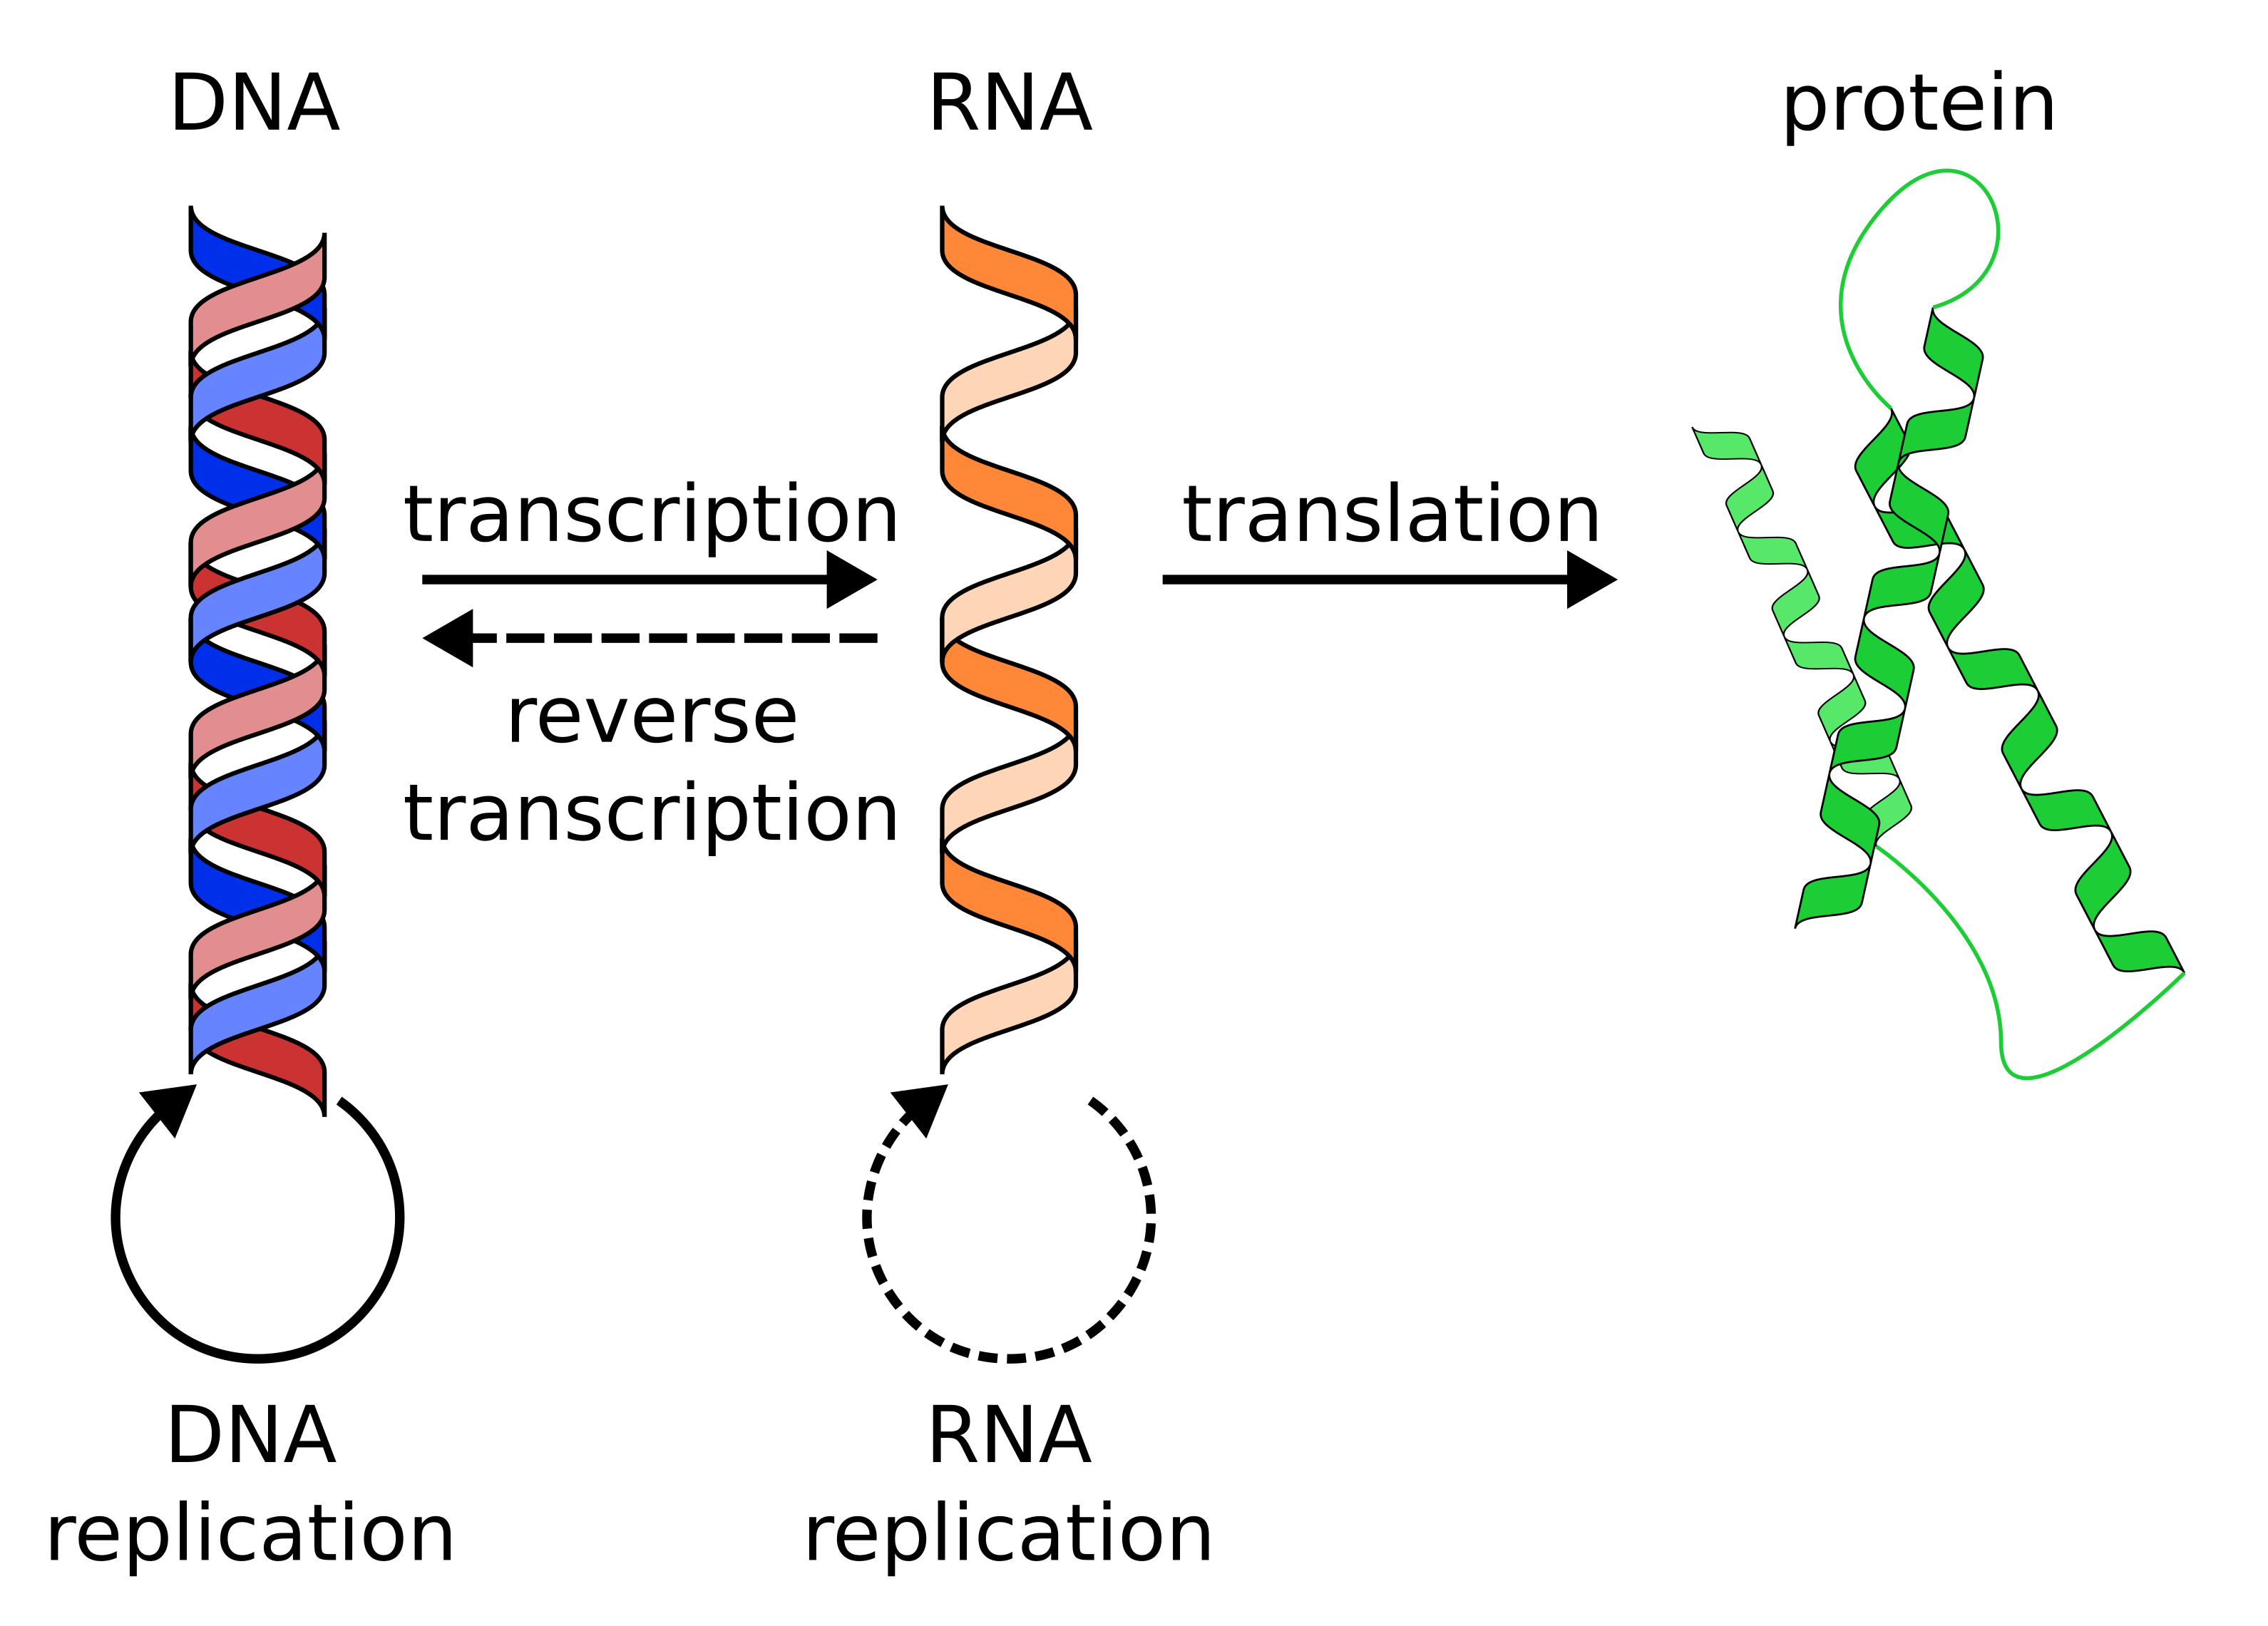
\includegraphics[width=\linewidth]{ch1.Introduction/imgs/central_dogma.png}
    \caption{The central dogma of molecular biology. Solid arrows indicate the general flow of information in the system, and dotted arrows special cases. TODO make mRNA RNA }
    \label{fig:central_dogma}
\end{figure}

The central dogma of molecular biology describes the flow of genetic information within a biological system. Whereas in a computer information is stored in bits, which can be either zero (0) or one (1), genetic information is stored in nucleotides, which can be either adenine (A), cytosine (C), guanine (G), or thymine (T). DNA, which stands for deoxyribonucleic acid, is composed of two large strands of these nucleotides that together form a double helix. Both strands contain the same information, but where there is a nucleotide A on one strand, there is always a corresponding nucleotide T on the other, and similarly for C and G. RNA, on the other hand, is a similar molecule but is typically single-stranded. It is transcribed from DNA and shares a similar nucleotide composition but replaces thymine (T) with uracil (U). RNA, as an intermediate molecule, plays a vital role in the central dogma of molecular biology, serving as the bridge between DNA and proteins. Through the process of translation, the information encoded in RNA is decoded and used to assemble amino acids in chains, ultimately resulting in the synthesis of proteins. Proteins carry out various tasks in our bodies, such as enabling chemical reactions, transporting other molecules, providing structure, and acting as regulators of transcription and translation of genes.

% \subsection{Transcription}

% \begin{figure}[hbtp]
%     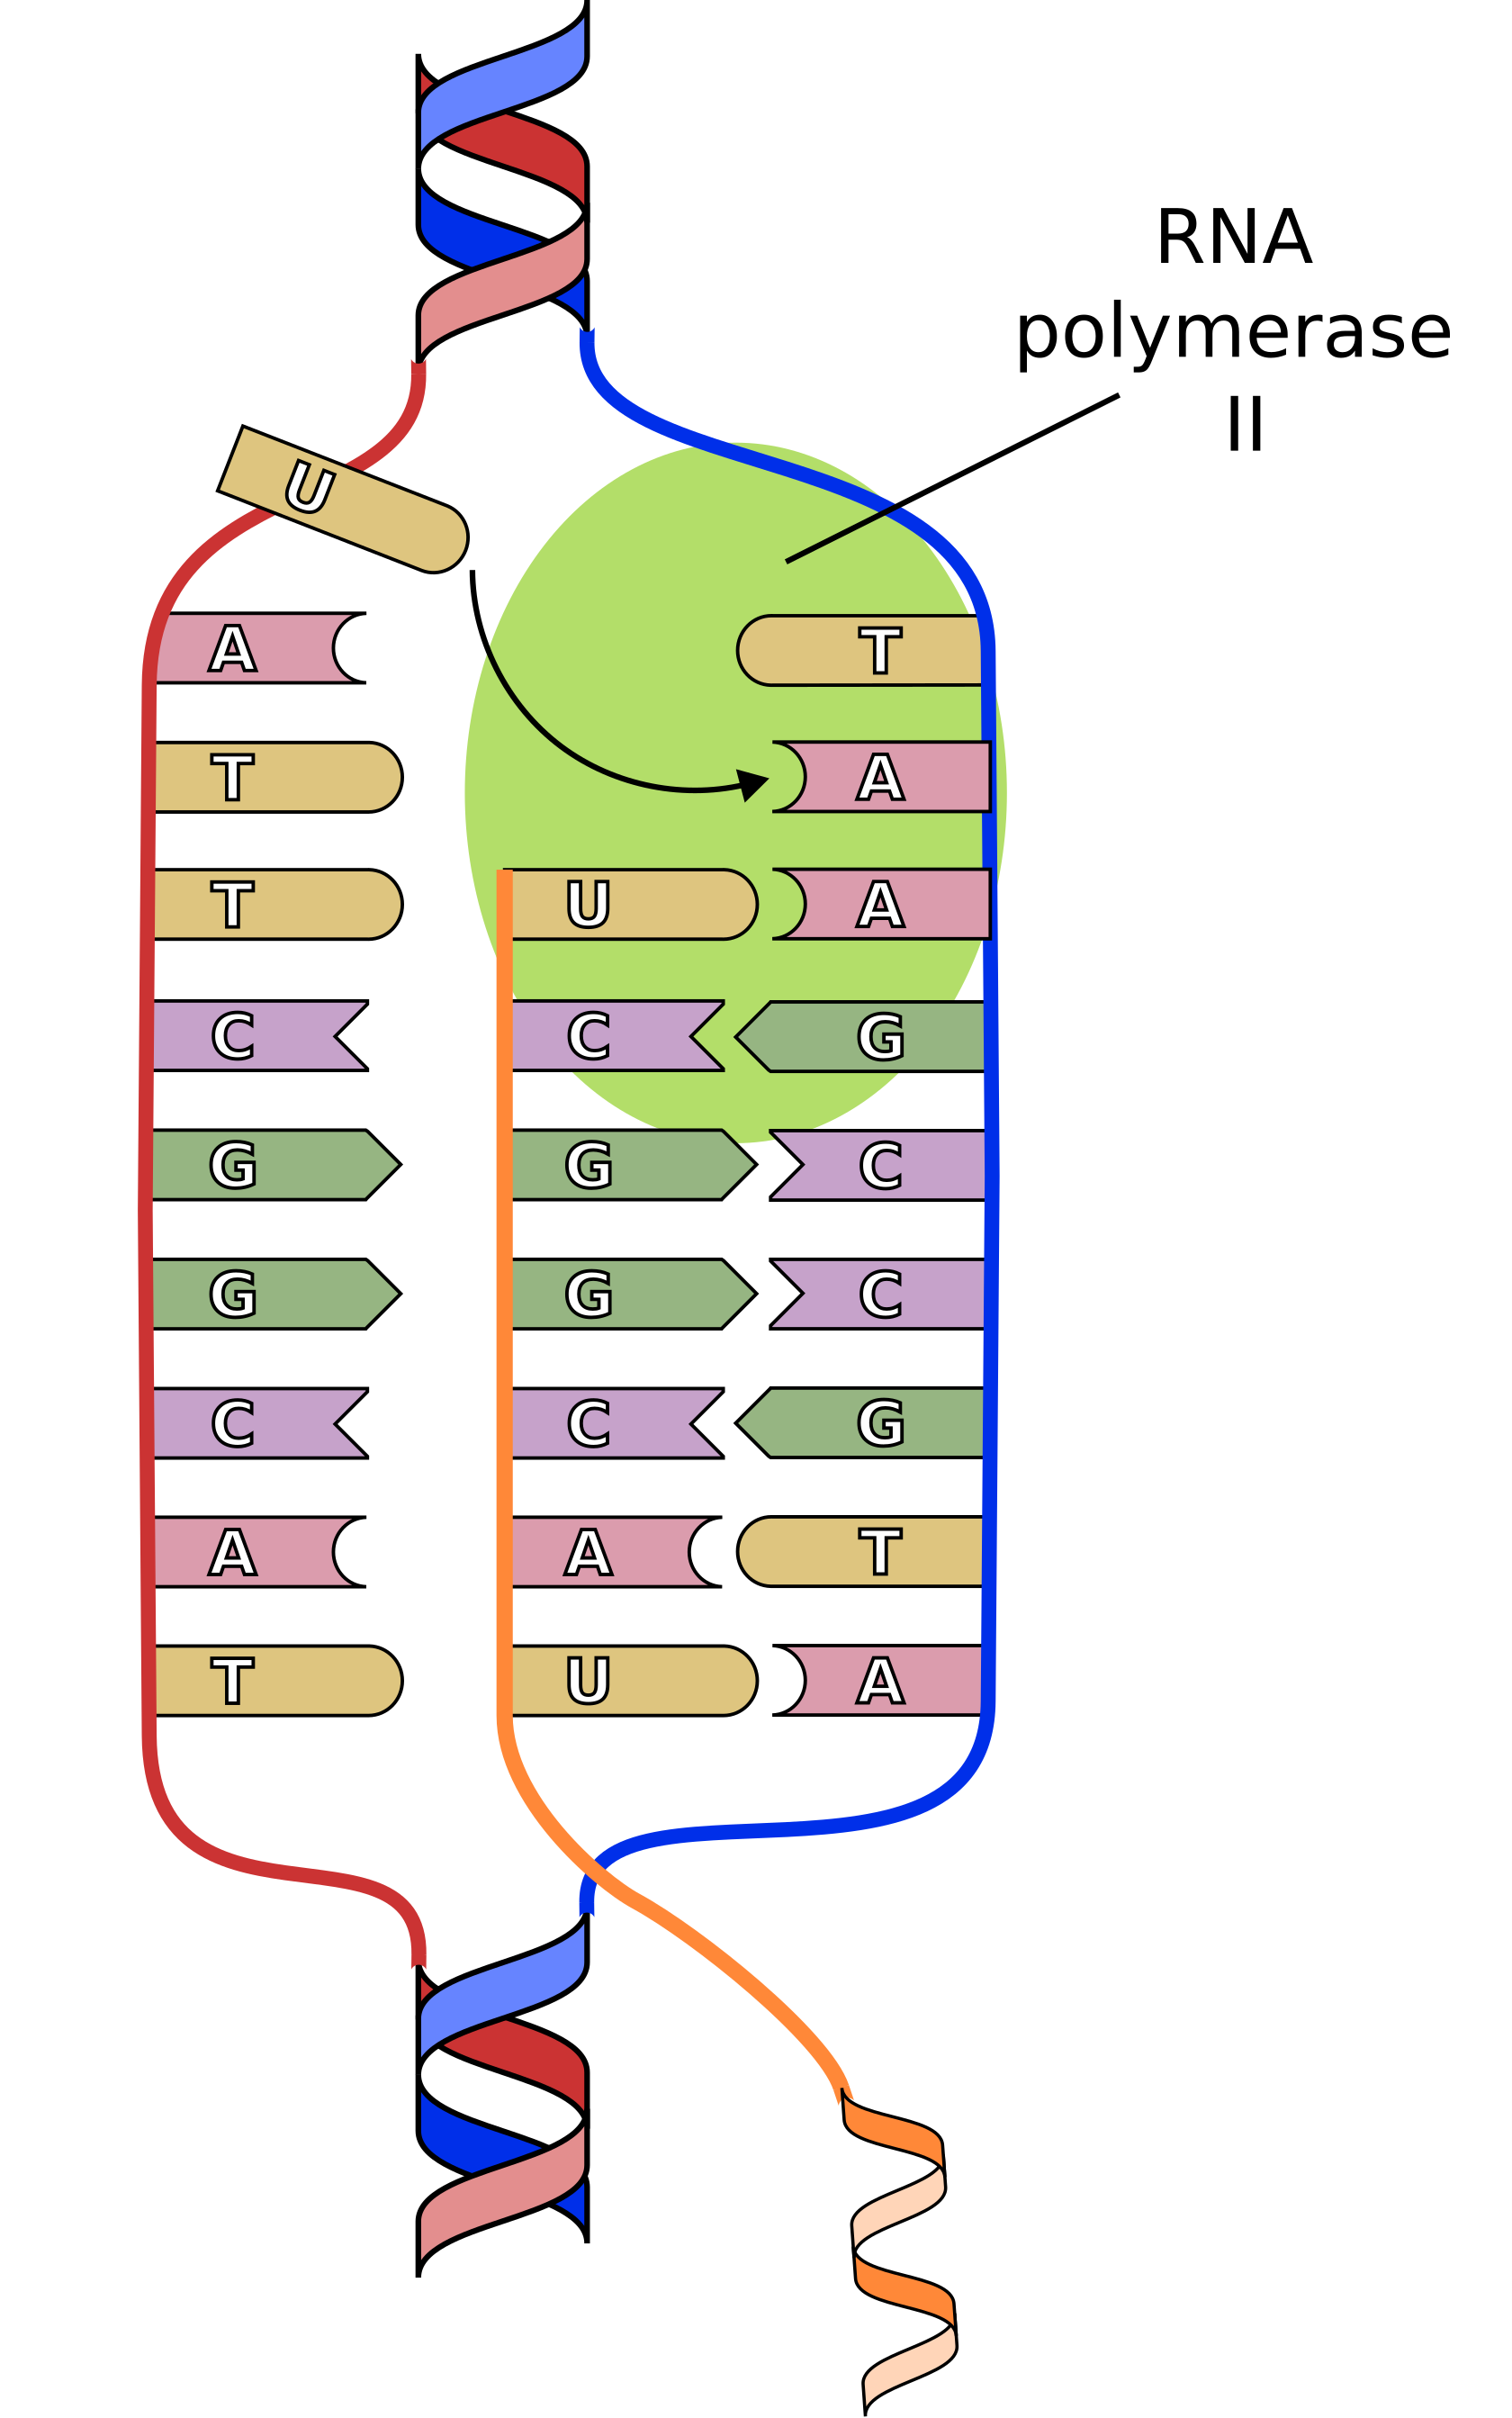
\includegraphics[height=0.5\textheight]{ch1.Introduction/imgs/transcription.png}
%     \caption{Caption}
%     \label{fig:transcription}
% \end{figure}

% \subsection{Translation}

% \begin{figure}[H]
%     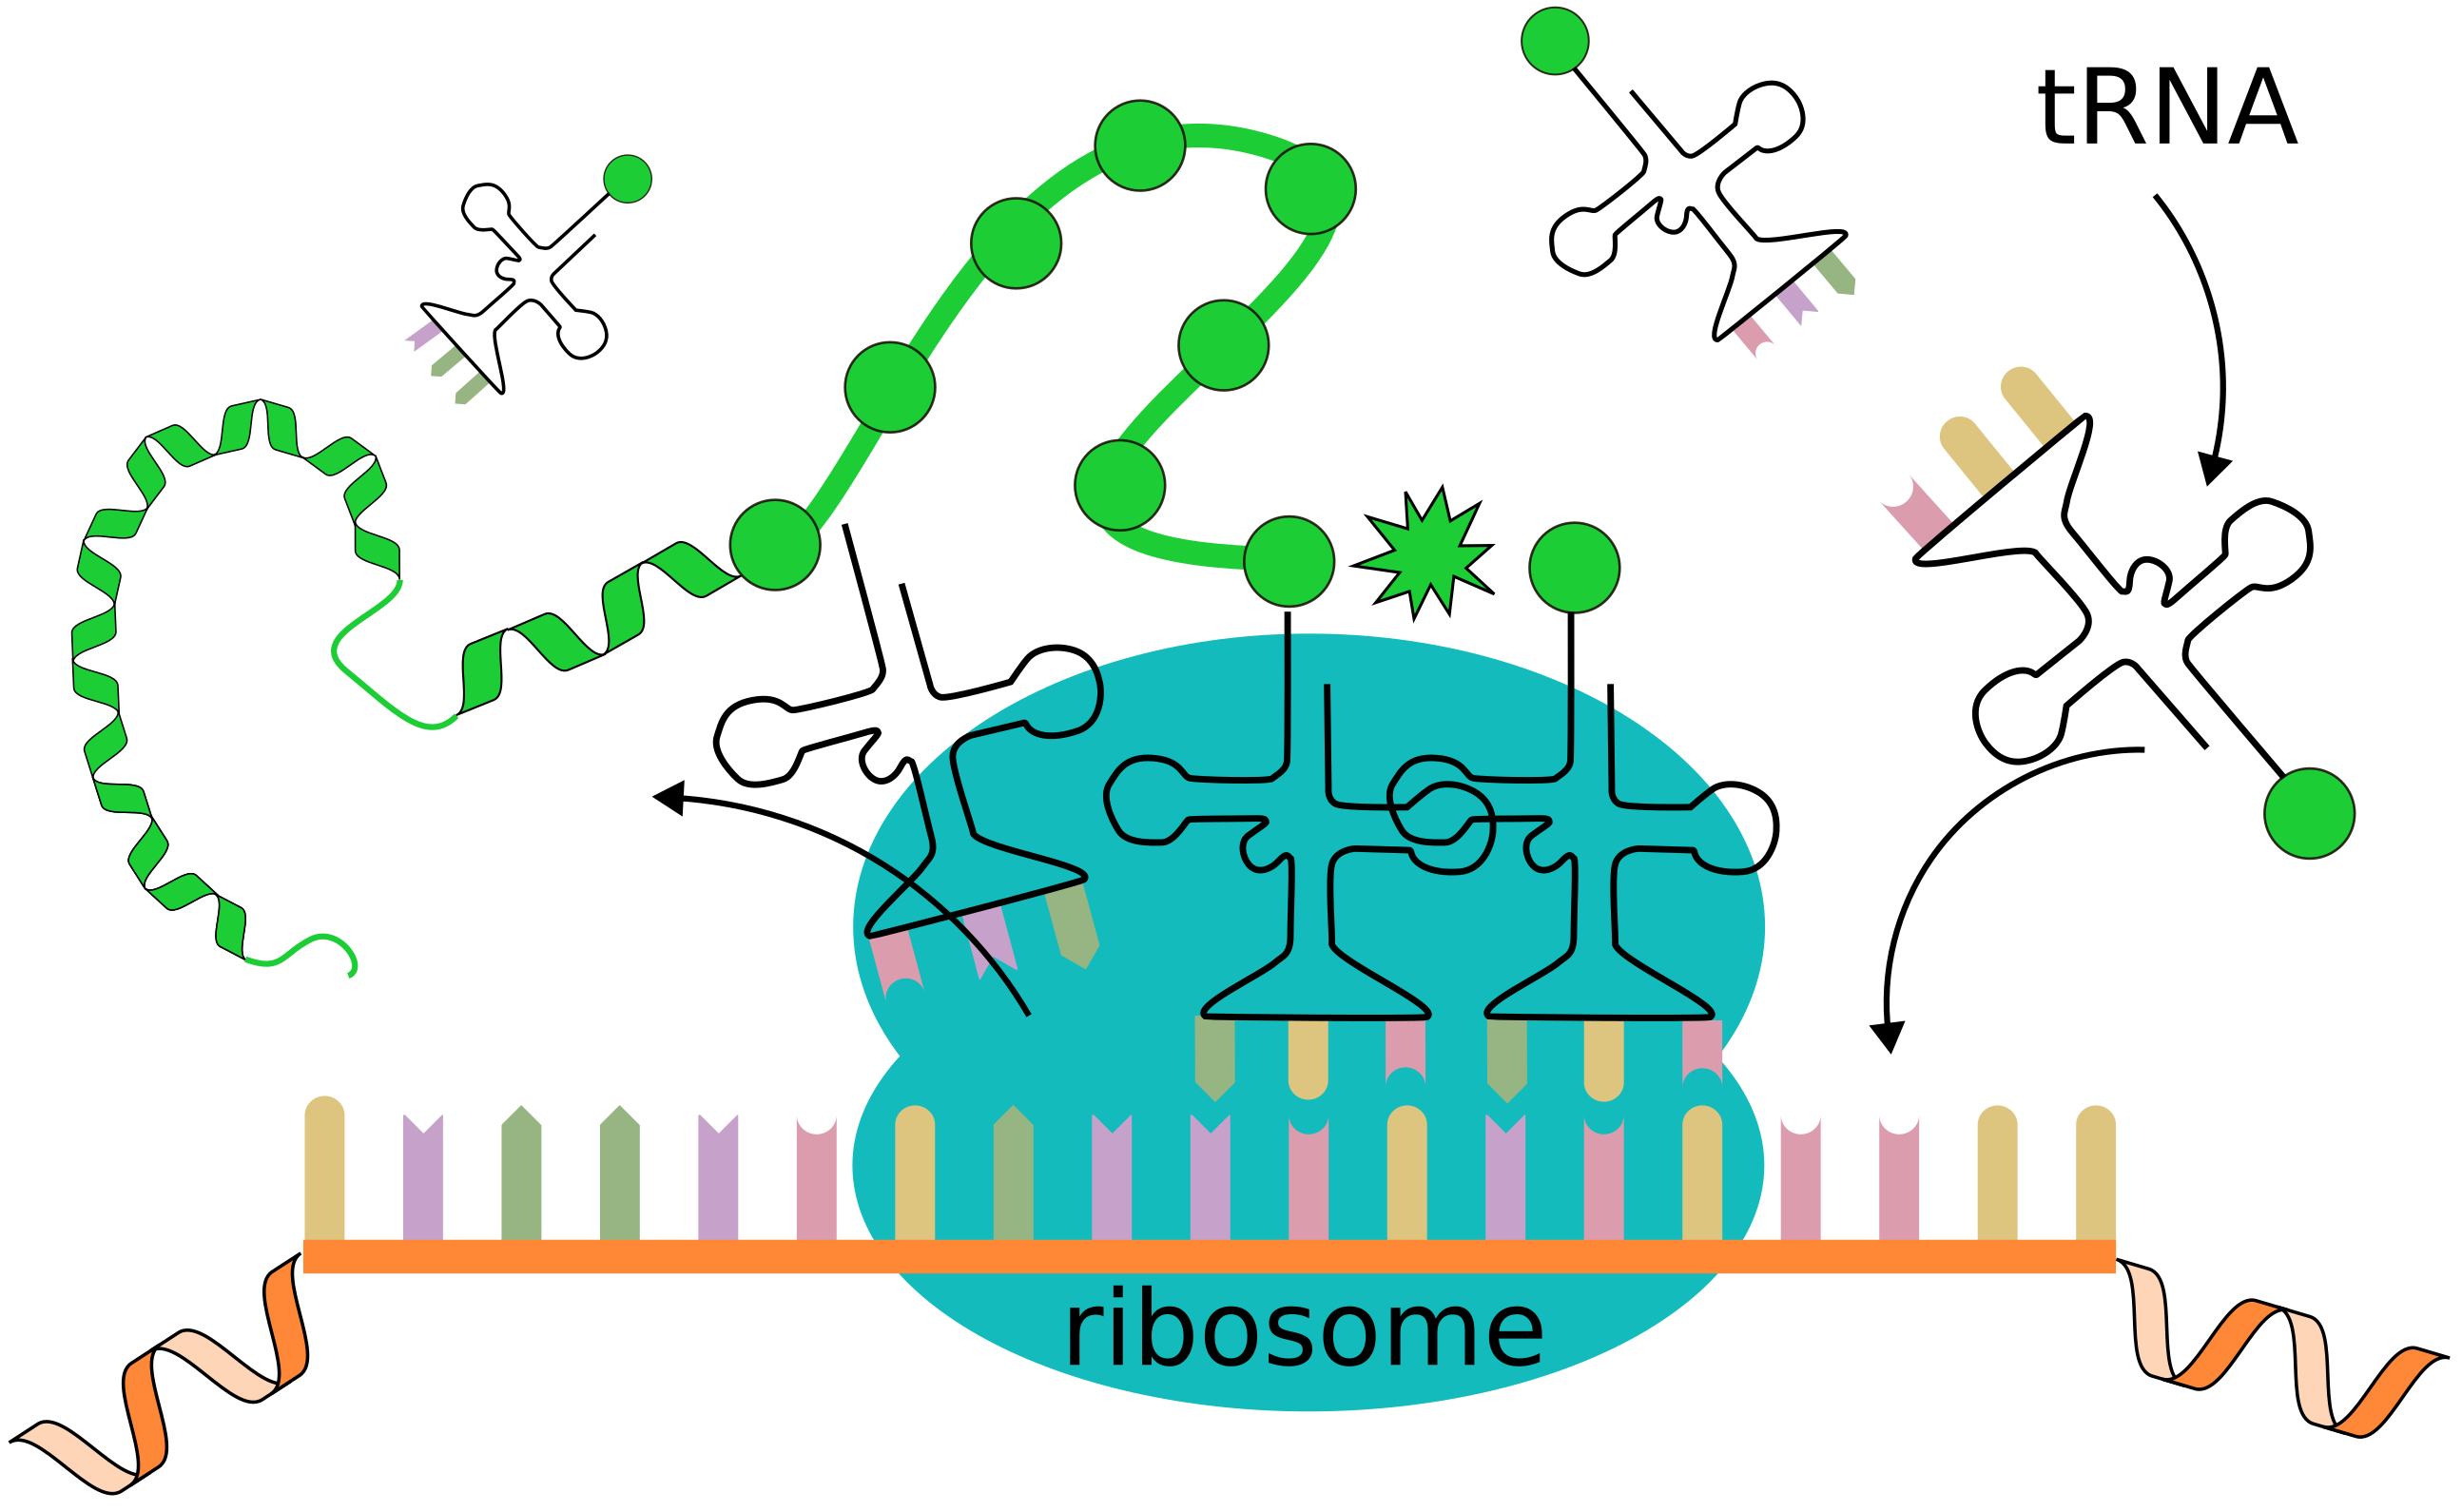
\includegraphics[width=\linewidth]{ch1.Introduction/imgs/translation.png}
%     \caption{Caption}
%     \label{fig:translation}
% \end{figure}

\section{Gene expression regulation}

A skin cell makes use of a completely different set of genes than a liver cell. This is possible due to the tight regulation of gene expression by these cells. To regulate their gene expression cells have a wide array of tools at their disposal. 

\subsection{Transcription Factors}

For a gene to be transcribed into

\subsection{Chromatin context}

\begin{figure}[H]
    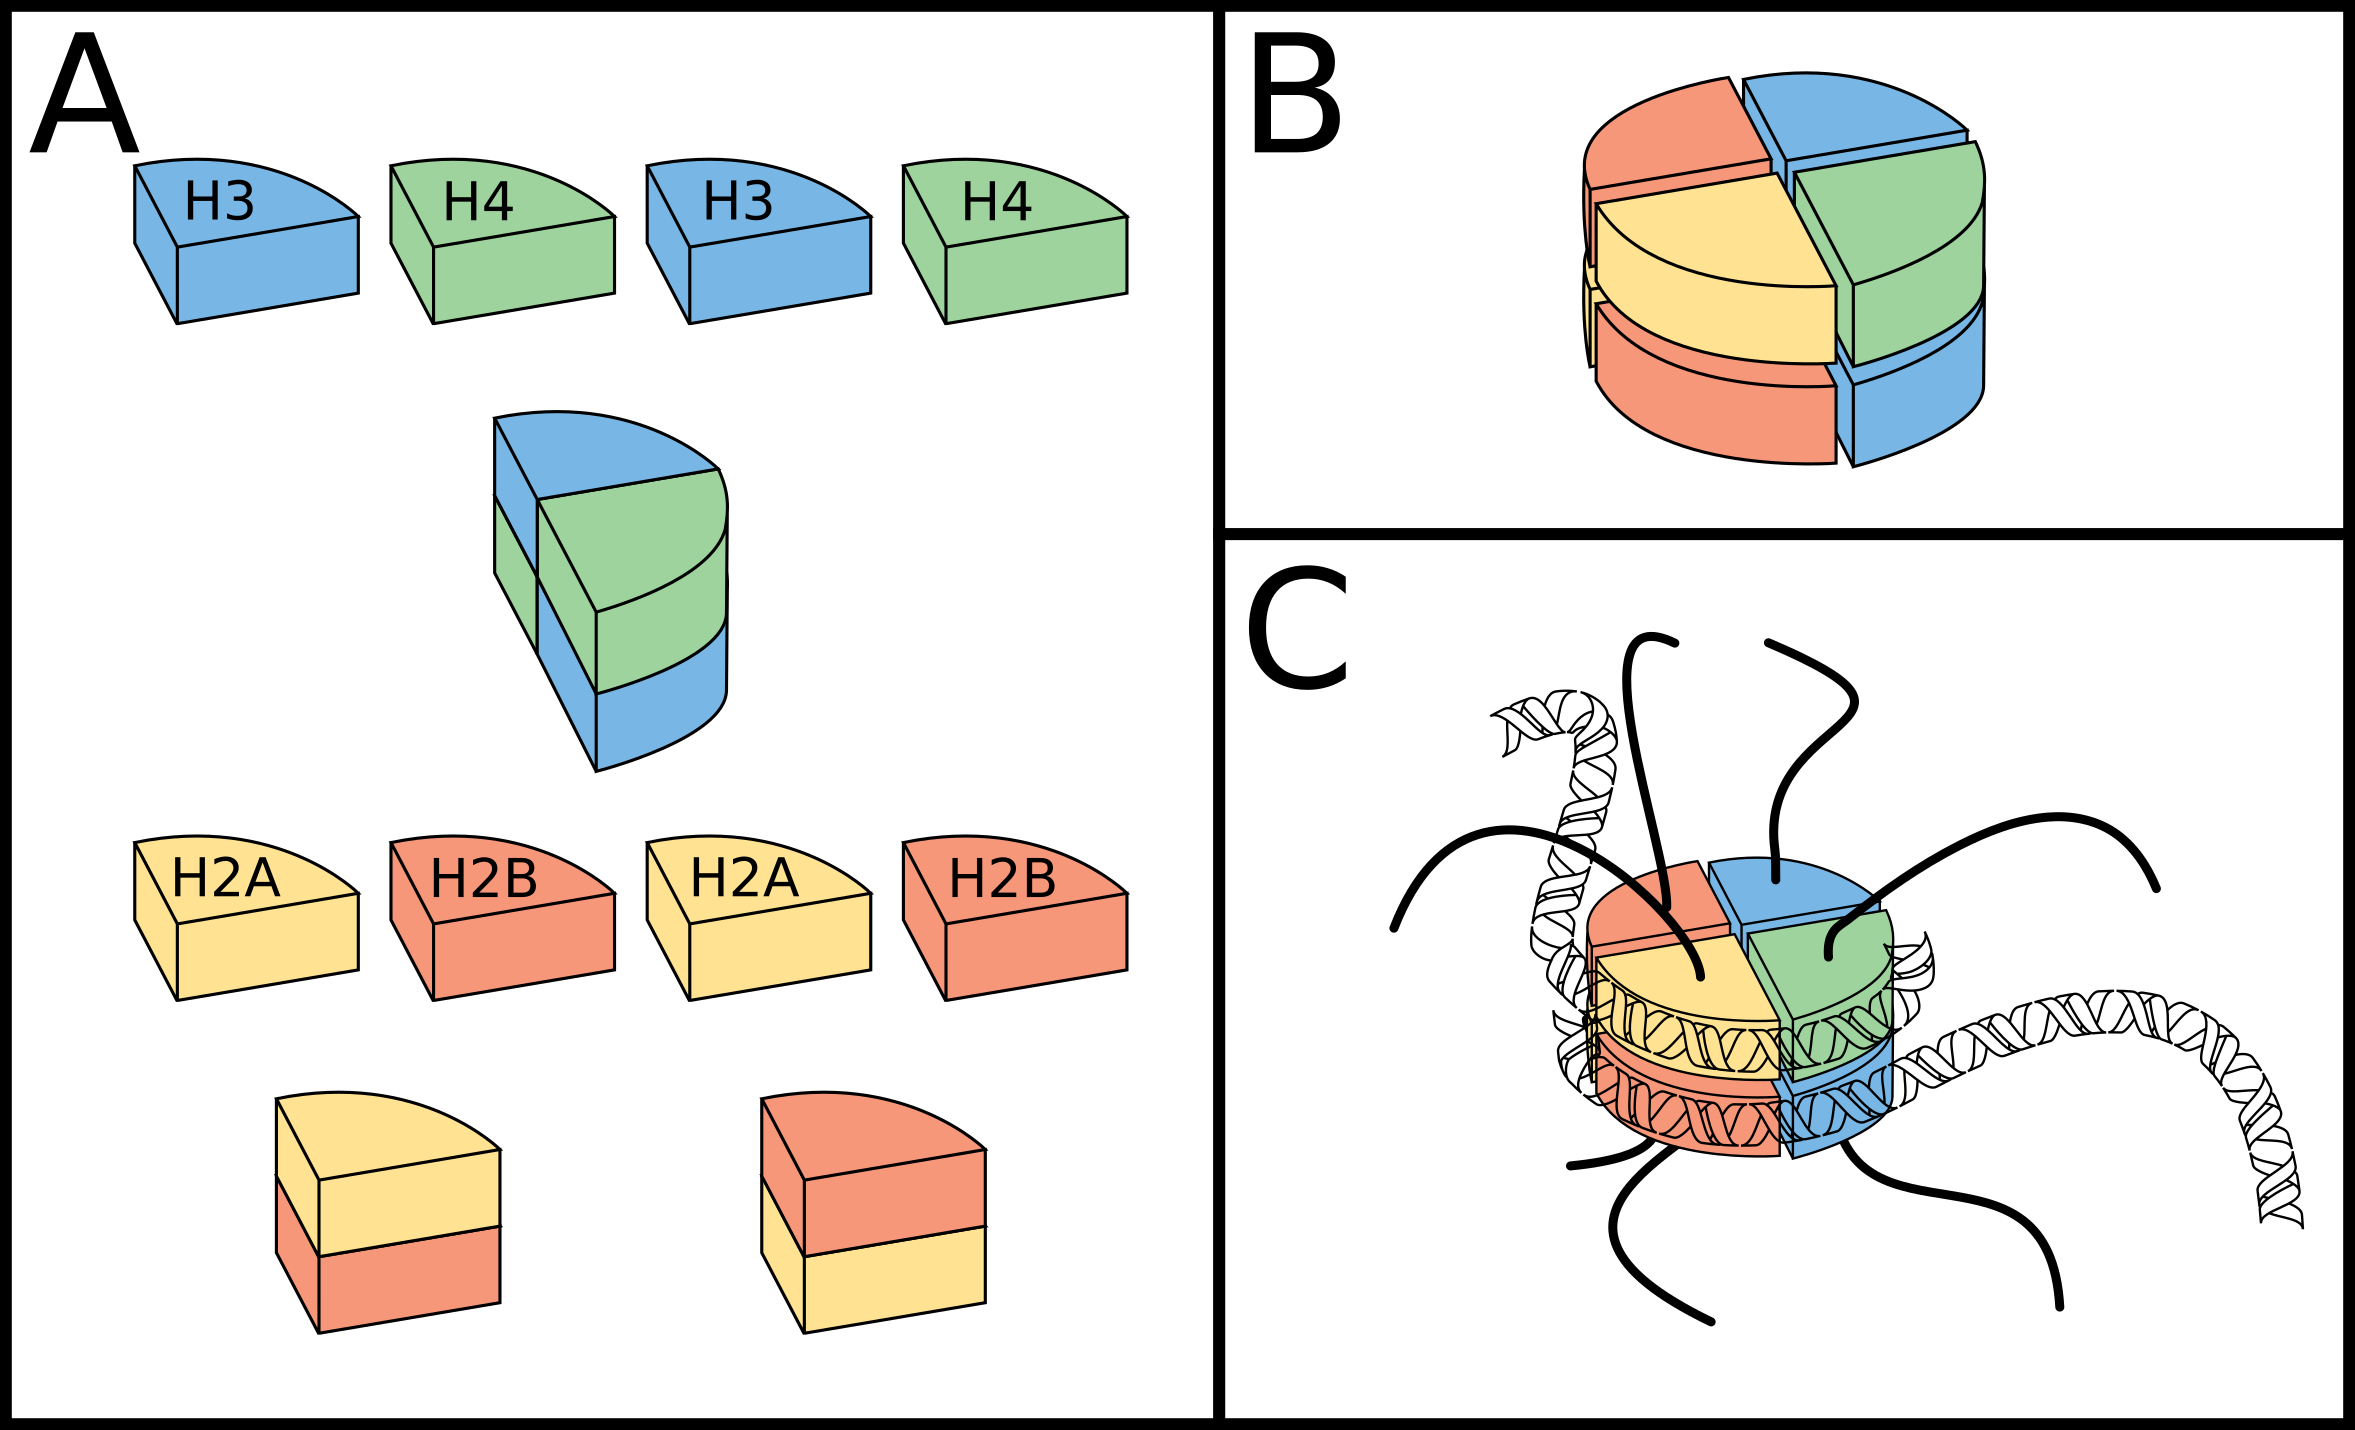
\includegraphics[width=\linewidth]{ch1.Introduction/imgs/histones.png}
    \caption{Caption}
    \label{fig:histones}
\end{figure}

\begin{figure}[hbtp]
    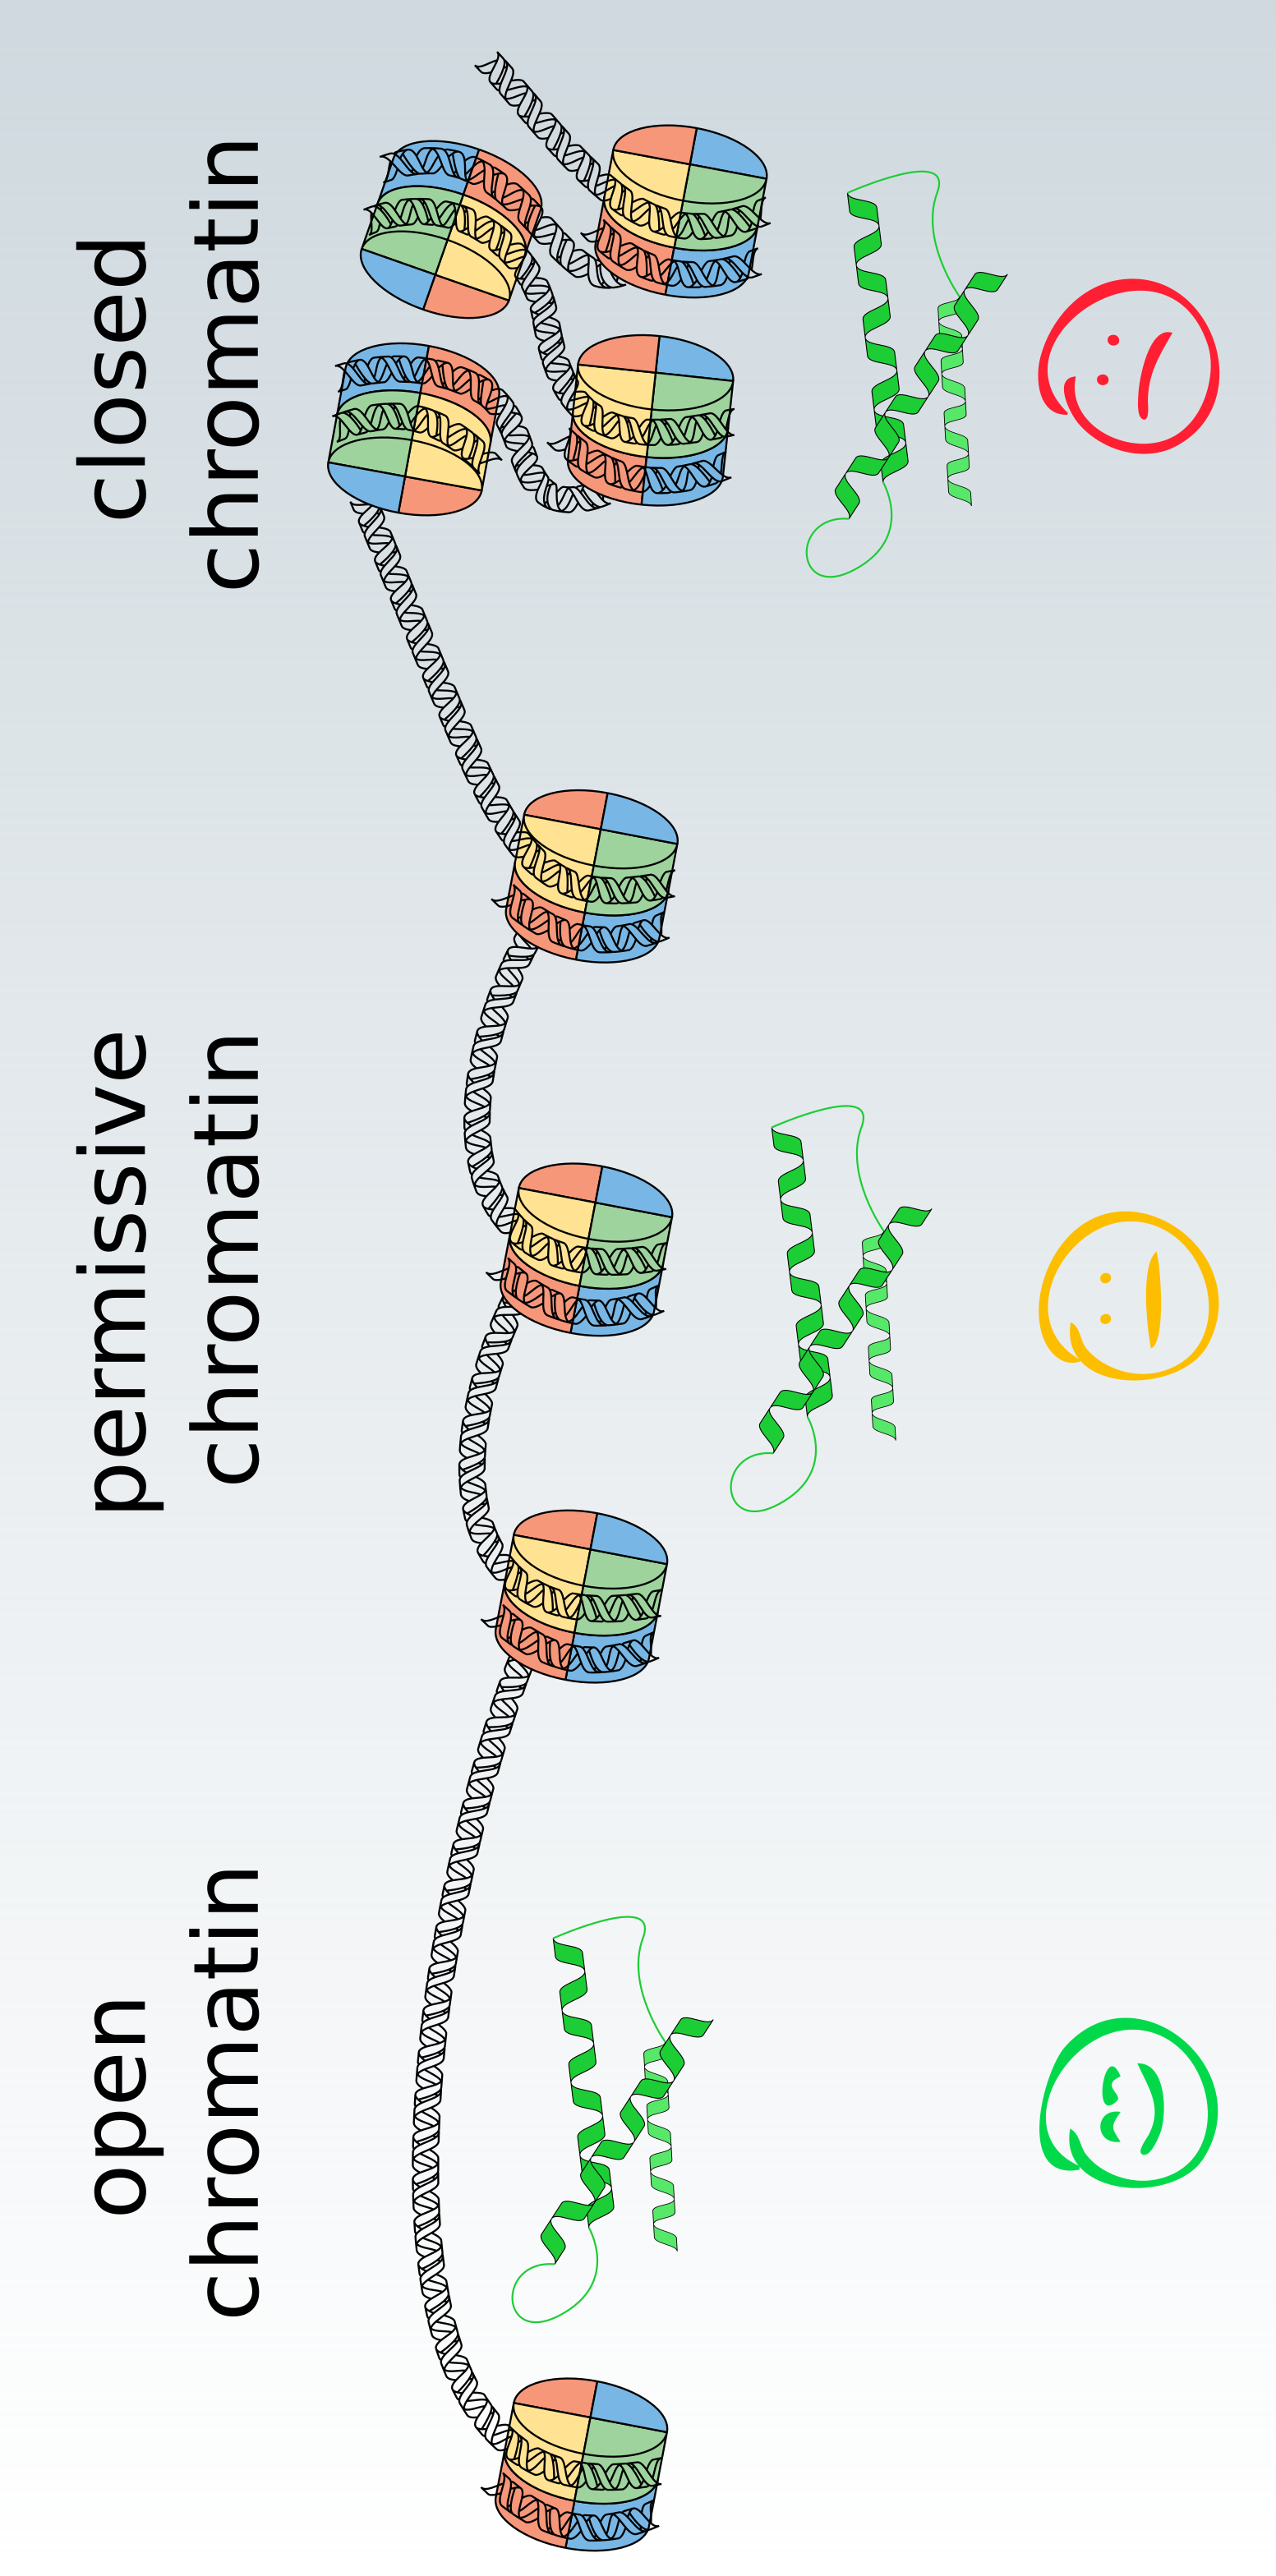
\includegraphics[height=0.9\textheight]{ch1.Introduction/imgs/accessibility.png}
    \caption{Caption}
    \label{fig:accessibility}
\end{figure}



\subsection{other gene regulatory modes}
% \subsubsection{mRNA degradation}
% \subsubsection{Post-transcriptional modification}
% \subsubsection{RNA transport}
% \subsubsection{Signal transduction}

\subsection{Gene regulatory networks}



\begin{figure}[H]
    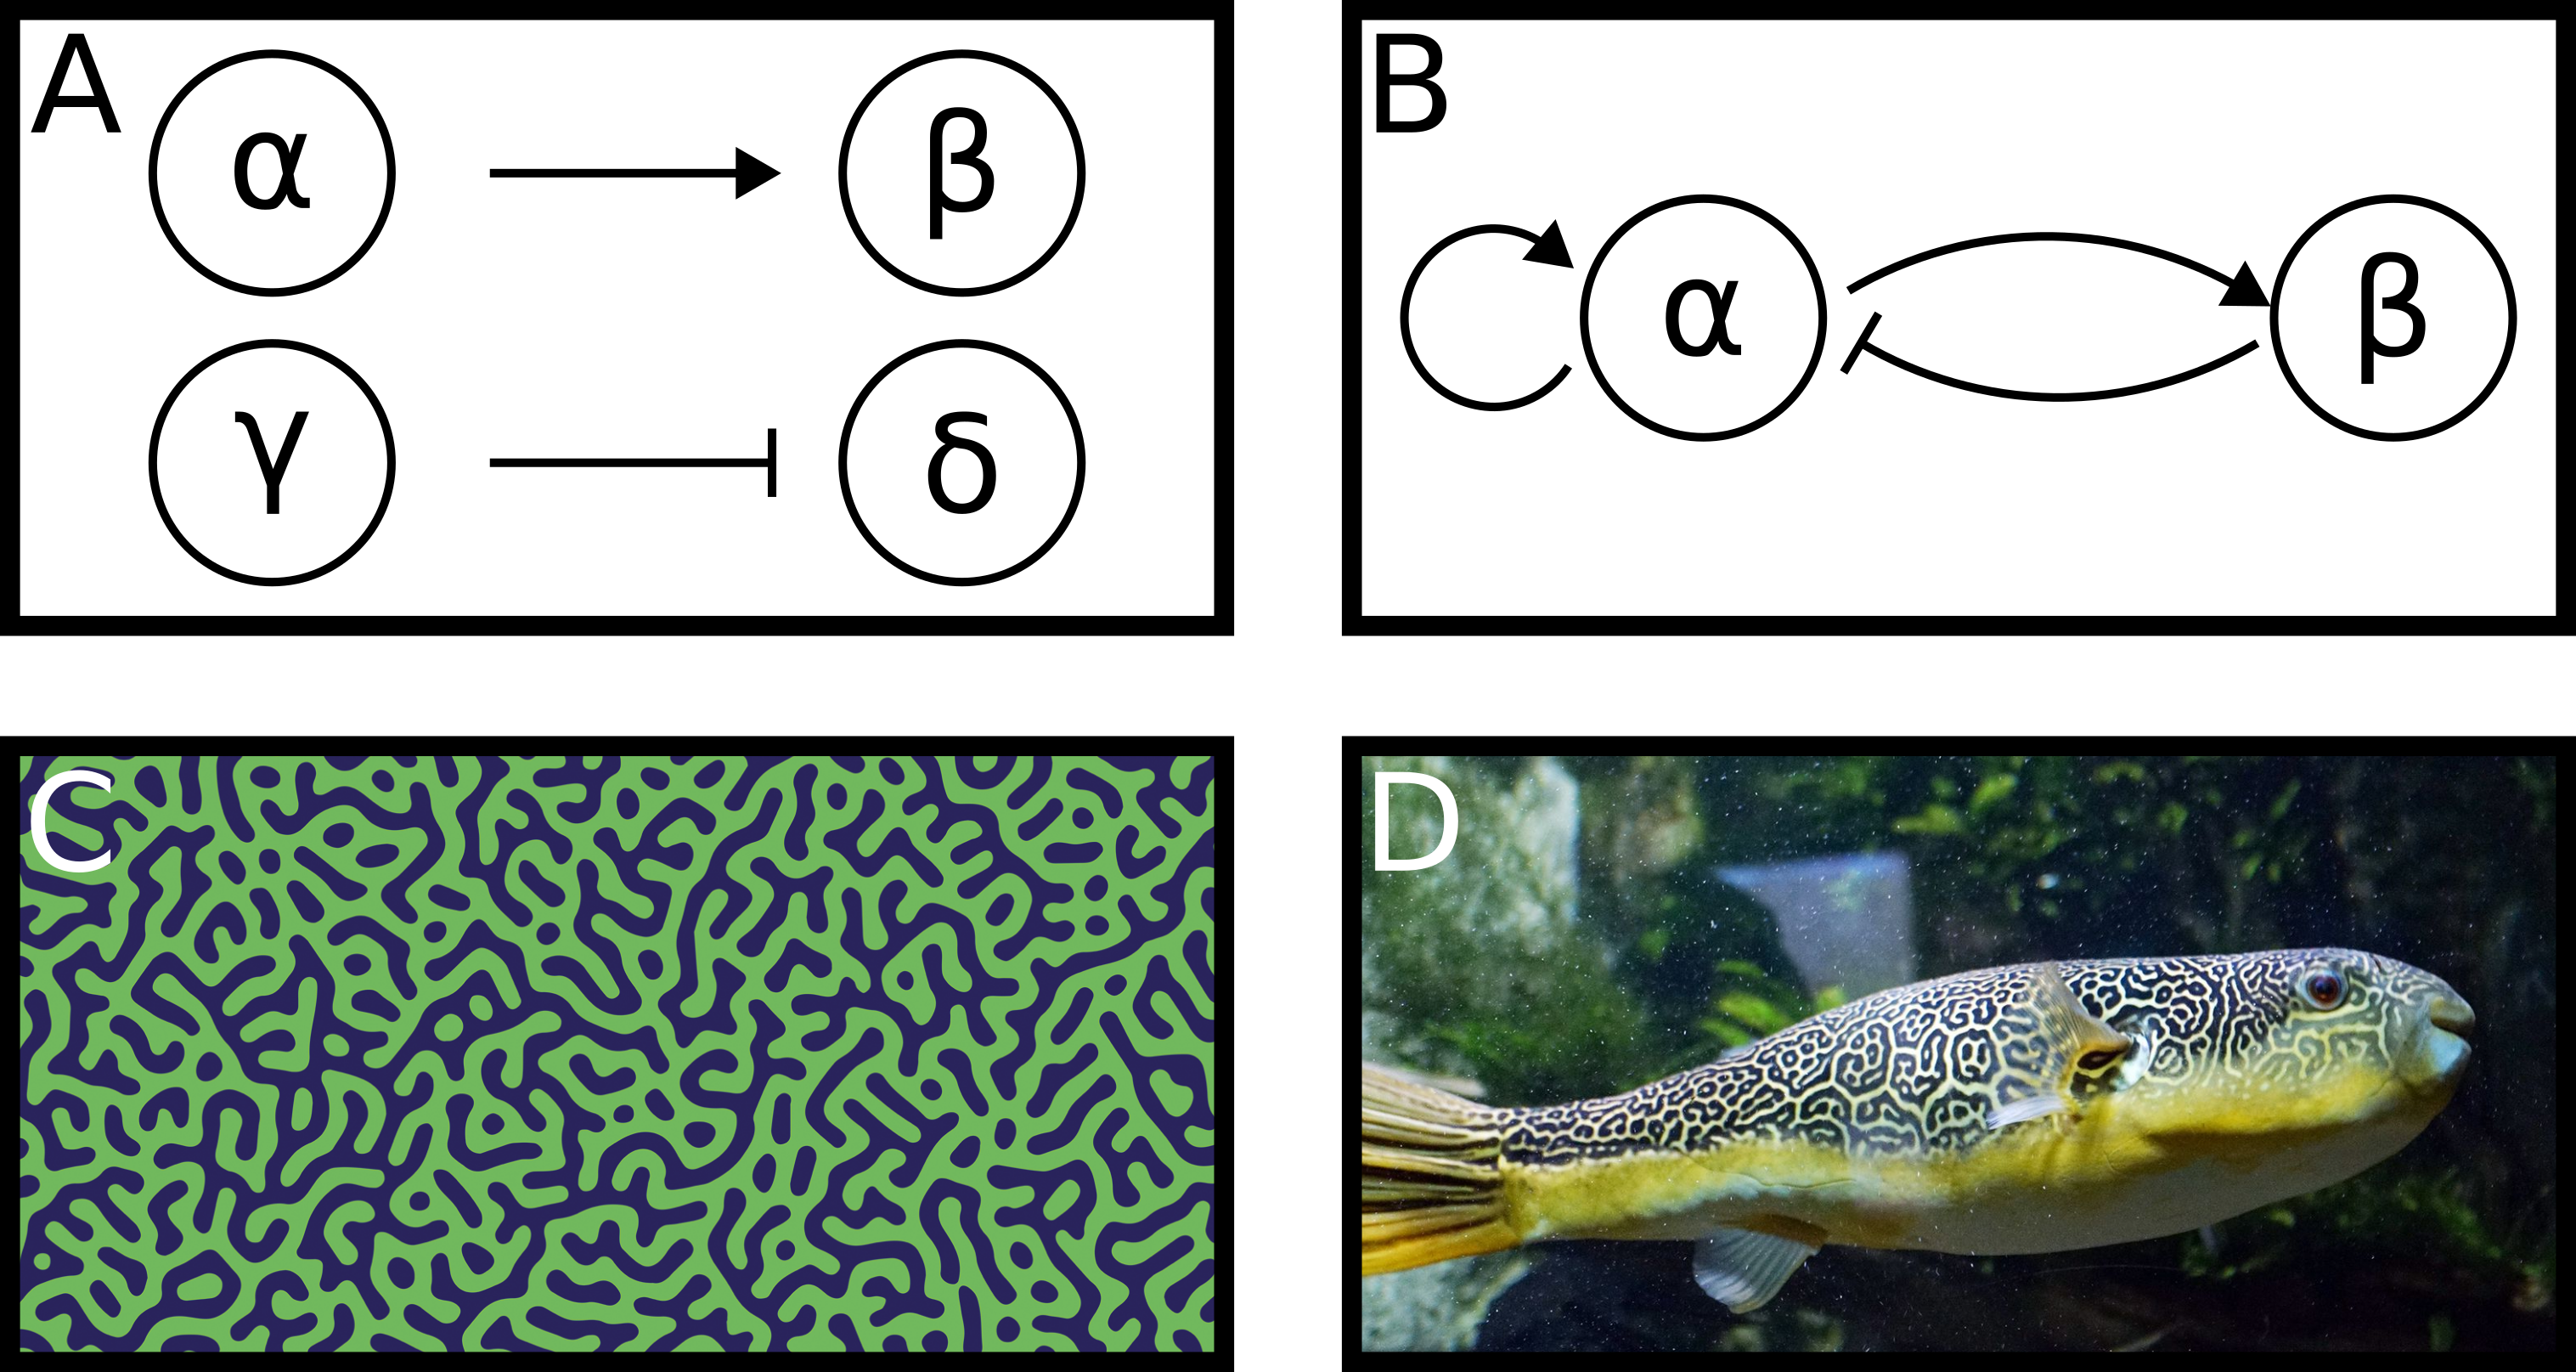
\includegraphics[width=\linewidth]{ch1.Introduction/imgs/network.png}
    \caption{(\textbf{A}) standard way of representing gene-gene interactions. Gene $\alpha$ upregulates gene $\beta$, and gene $\gamma$ downregulates gene $\delta$. (\textbf{B}) Gierer-Meinhardt gene regulatory network, where gene $\alpha$ upregulates itself and gene $\beta$, and gene $\beta$ downregulates gene $\alpha$. (\textbf{C}) Simulation of the Gierer-Meinhardt gene regulatory network in a spatial context. (\textbf{D}) A Mbuna pufferfish with Turing pattern. Image taken from Tiia Monto from https://en.wikipedia.org/wiki/Mbu\_pufferfish\#/media/File:Tetraodon\_mbu\_2.jpg}
    \label{fig:network}
\end{figure}

\section{Evolution}

\begin{figure}[H]
    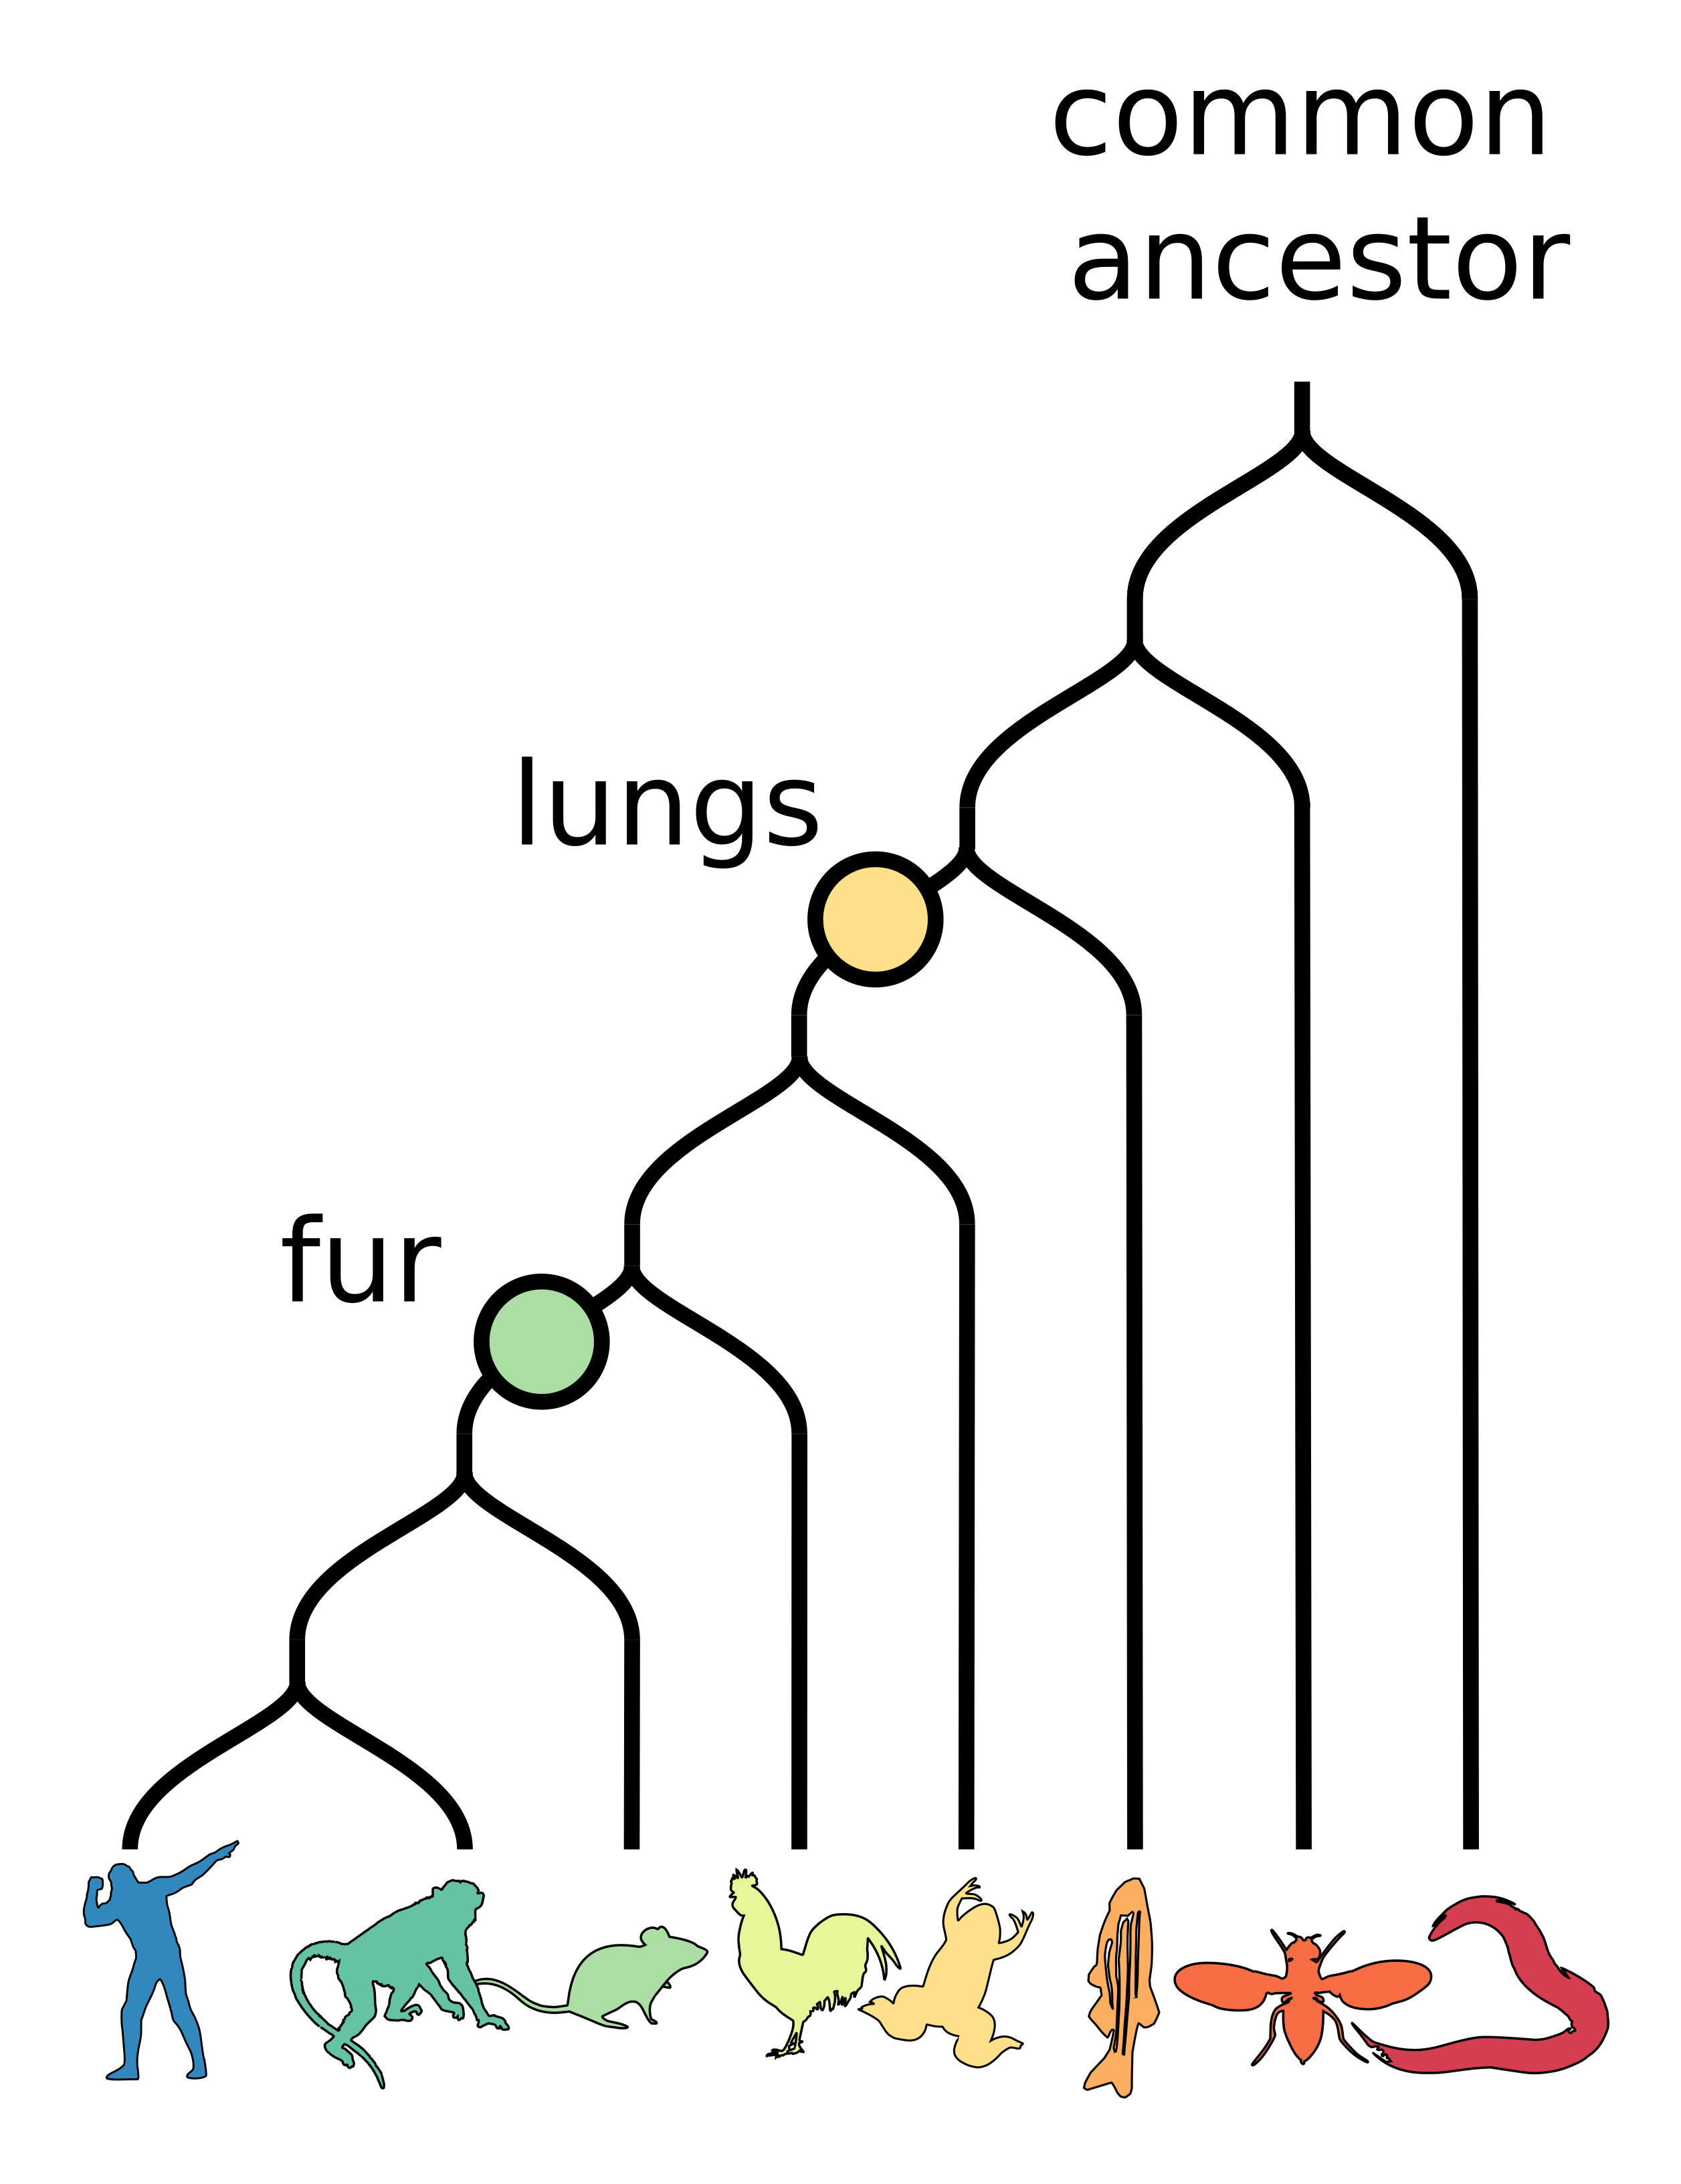
\includegraphics[width=0.5\linewidth]{ch1.Introduction/imgs/phylogeny.png}
    \caption{caption}
    \label{fig:phylogeny}
\end{figure}

\section{Development}

A single fertilized human egg cell develops into a complex collection of 37 trillion cells by the time the individual reaches adulthood. All the information necessary for this development is present at fertilization. How does each cell know what to develop into? Apart from sensing its direct neighborhood, all the information is contained.

\section{Evolutionary development (evo-devo)}



\subsection{evo-devo gene toolkit}

\subsection{The hourglass model and the phylotypic stage}

\begin{figure}[H]
    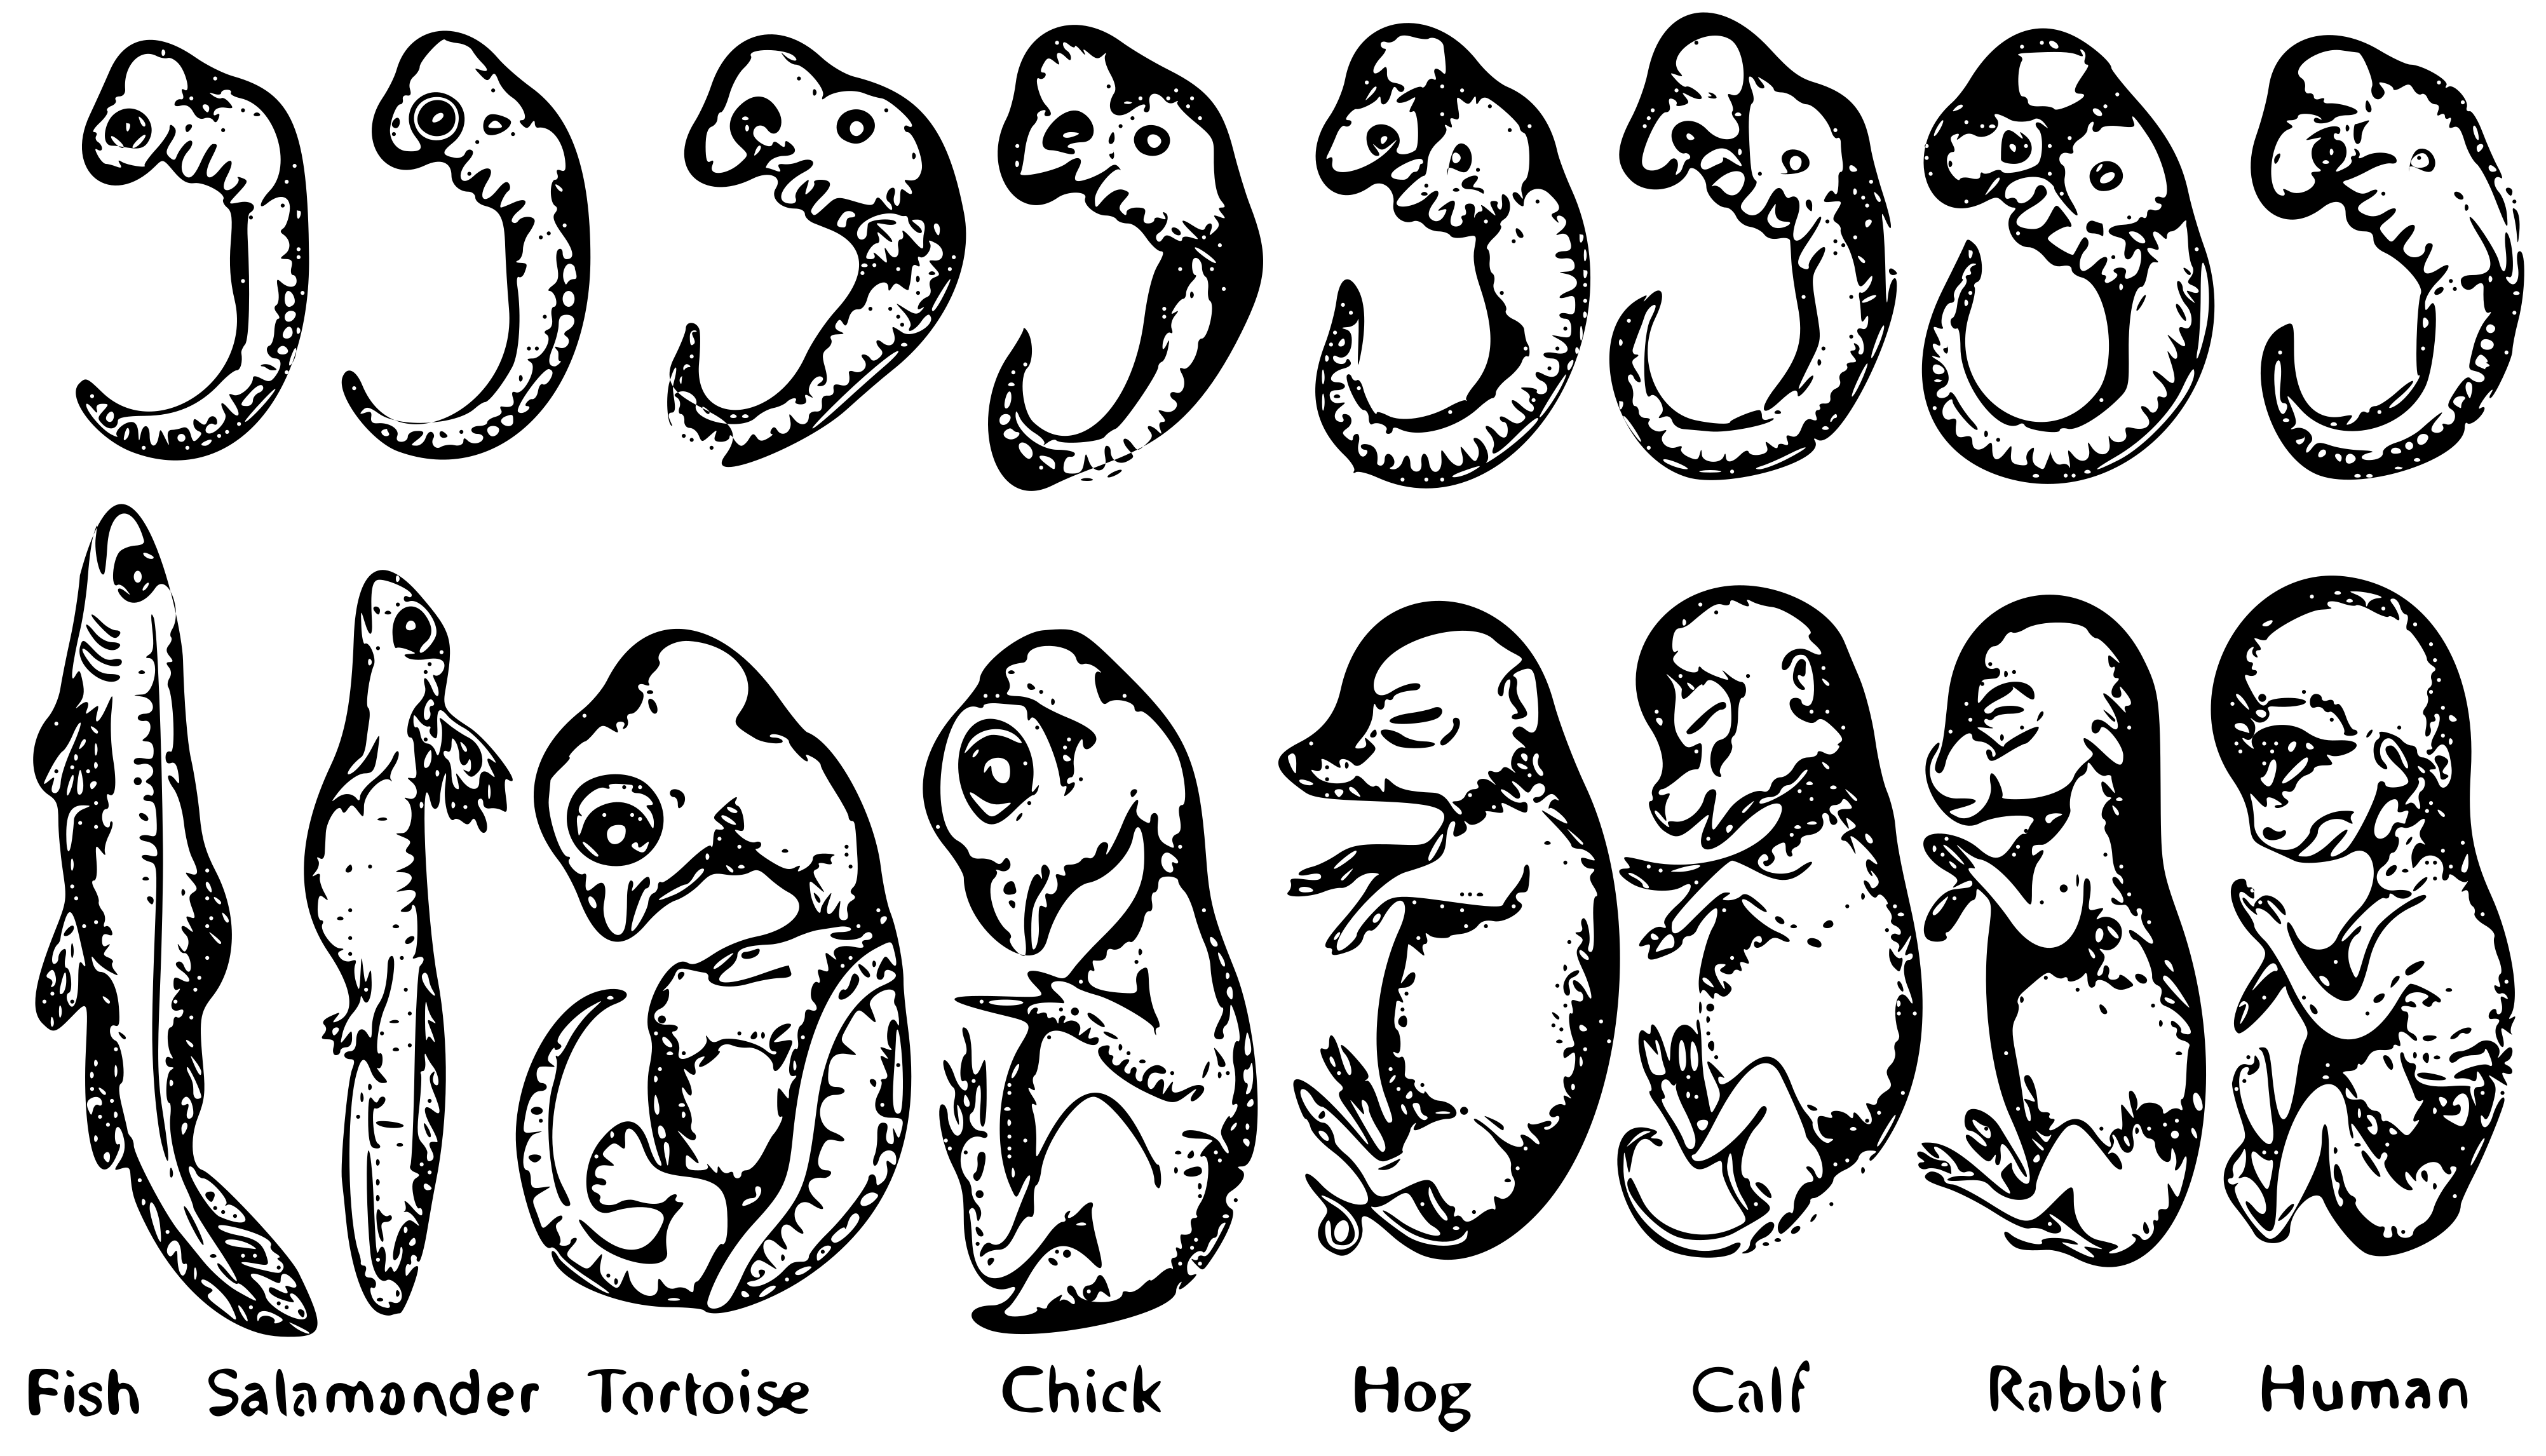
\includegraphics[width=\linewidth]{ch1.Introduction/imgs/haeckel.png}
    \caption{caption}
    \label{fig:haeckel}
\end{figure}

\section{Computational biology}

The field of computational biology concerns itself with the analysis of the enormous quantities of data that molecular biology produces. 

\begin{figure}[H]
    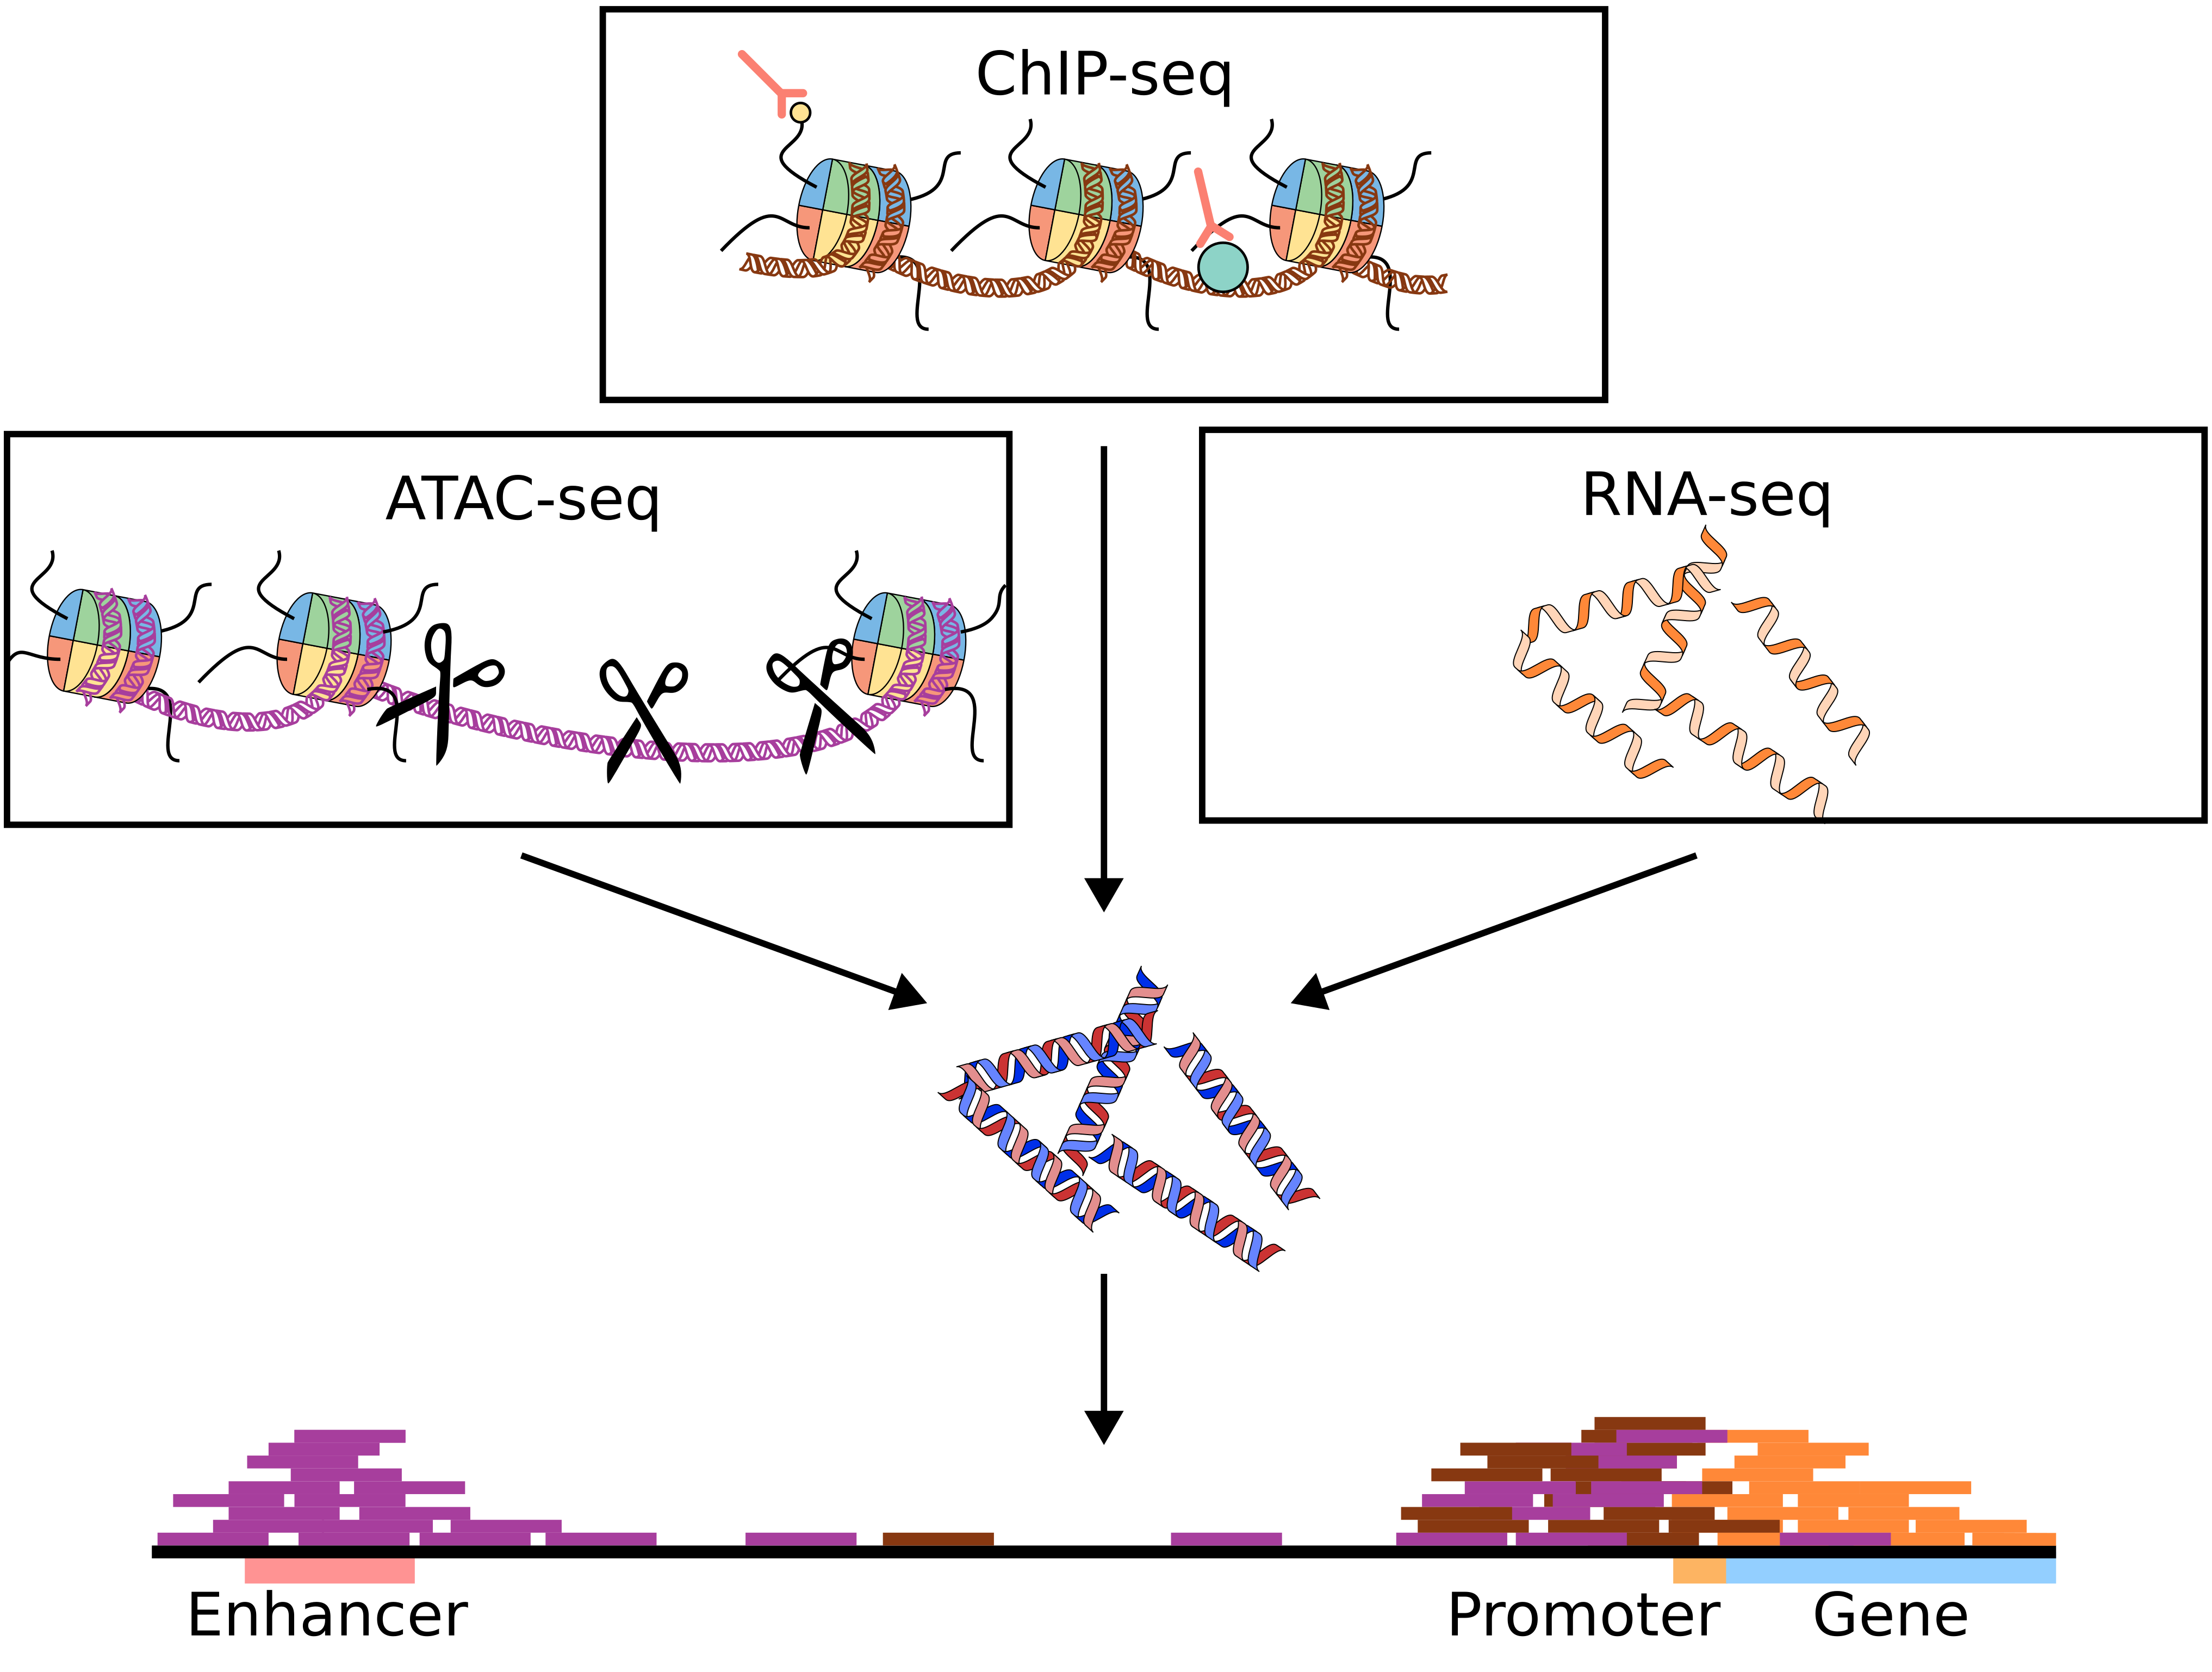
\includegraphics[width=\linewidth]{ch1.Introduction/imgs/analysis.png}
    \caption{caption}
    \label{fig:analysis}
\end{figure}

\subsection{Single cell}

\section{Thesis overview}
